%%%%%%%%%%%%%%%%%%%%%%%%%%%%%%%%%%%%%%%%%
% Presentation Template
% LaTeX Template
% Version 1.0 (2023-02-08)
%
% This template was adapted by:
% Jonathan Decker (jonathan.decker@uni-goettingen.de)
% From a template made by:
% Julian Kunkel (julian.kunkel@gwdg.de)
%
%%%%%%%%%%%%%%%%%%%%%%%%%%%%%%%%%%%%%%%%%
\documentclass[compress,aspectratio=169]{beamer}

% make sure the theme file is on this path
\usepackage{../assets/beamerthemeGoettingen}

\addbibresource{ref.bib}
\graphicspath{{../}{../assets/}}

% --- document configuration ---
\newcommand{\mytitle}{Evaluation of Time-Series Databases}
% Leave empty for no subtitle
\newcommand{\mysubtitle}{Elasticsearch and InfluxDB}
\newcommand{\myauthor}{Lars Quentin}
\newcommand{\myauthorurl}{https://lquenti.de/}
\newcommand{\myvenue}{HPCSA}
% For example, use \today
\newcommand{\mydate}{\today}
% For example, Institute for Computer Science / GWDG
\newcommand{\myinstitute}{University of G\"ottingen}

\configuretitlepage

\begin{document}

\begin{frame}[plain]
	\titlepage
\end{frame}

\begin{frame}[t]{Table of Contents}
  \tableofcontents[subsectionstyle=hide/hide]
\end{frame}

% --- slides begin ---

\section[Introduction]{Getting up to Speed: Introduction}
\begin{frame}{Why do we care about Time Series Metrics Data?}
\begin{columns}[T]
\begin{column}{0.5\textwidth}
\begin{itemize}
  \item Usage Overview
  \item Find Bottlenecks
  \item Help with Workload Balancing
  \item Demand Analysis and Forecasting
  \item Optimize Energy Efficiency
\end{itemize}
~\\~\\
\pause
But why do we care about performance?
\end{column}
\begin{column}{0.5\textwidth}
\begin{figure}
  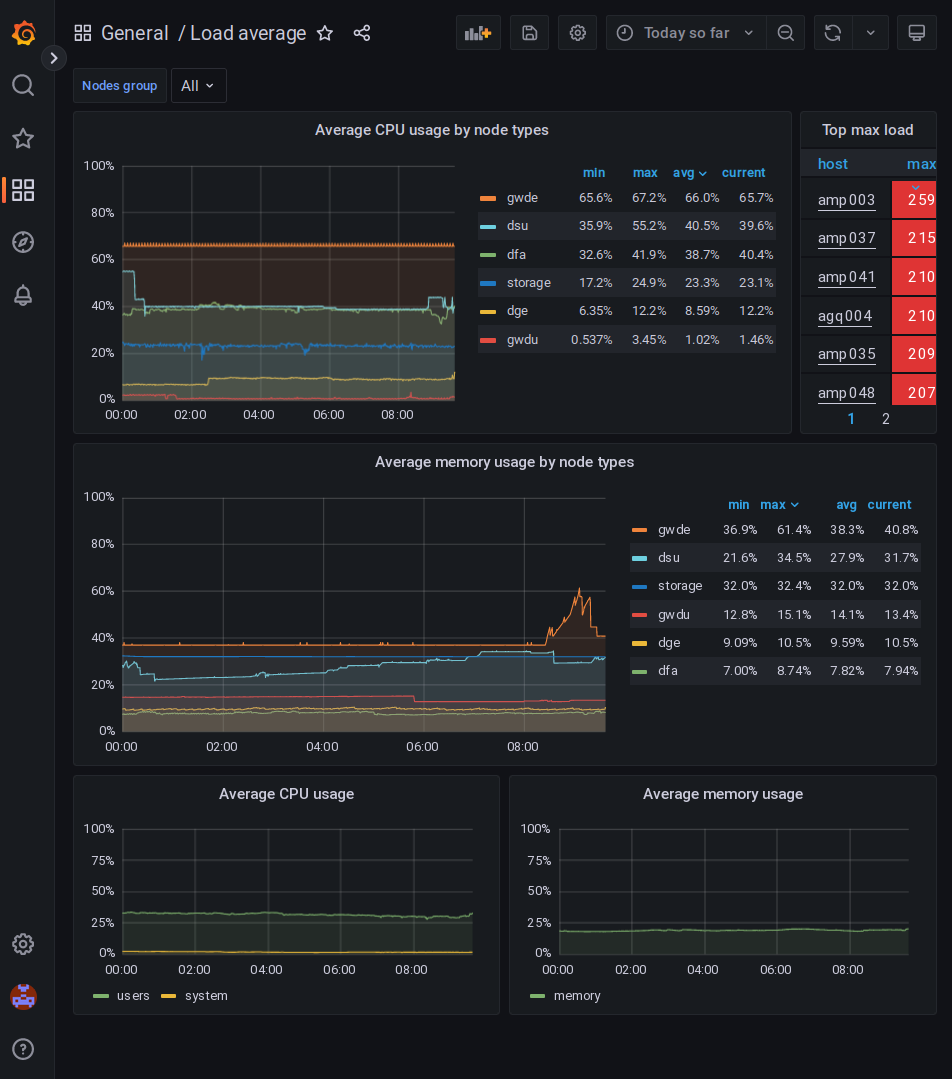
\includegraphics[height=.8\textheight]{example_grafana_dashboard.png}
\end{figure}
\end{column}
\end{columns}
\end{frame}

\begin{frame}{Monitoring System Architecture}
\begin{center}
\begin{figure}
  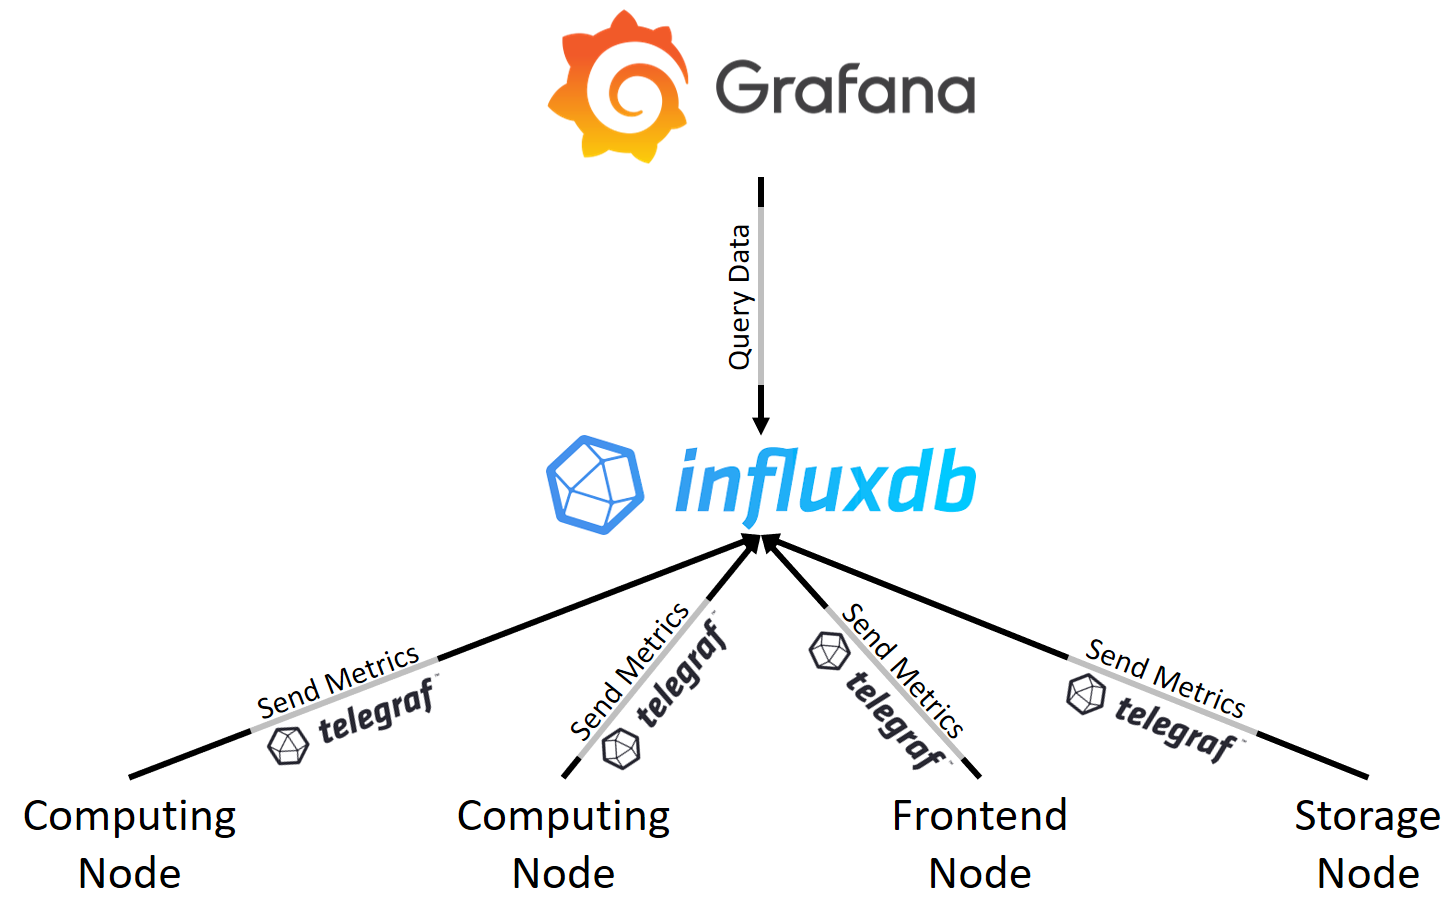
\includegraphics[height=.8\textheight]{assets/monitoring_system_architecture.png}
  \caption{Monitoring System Architecture}
\end{figure}
\end{center}
\end{frame}

\begin{frame}{But actually...}
\begin{center}
\begin{figure}
  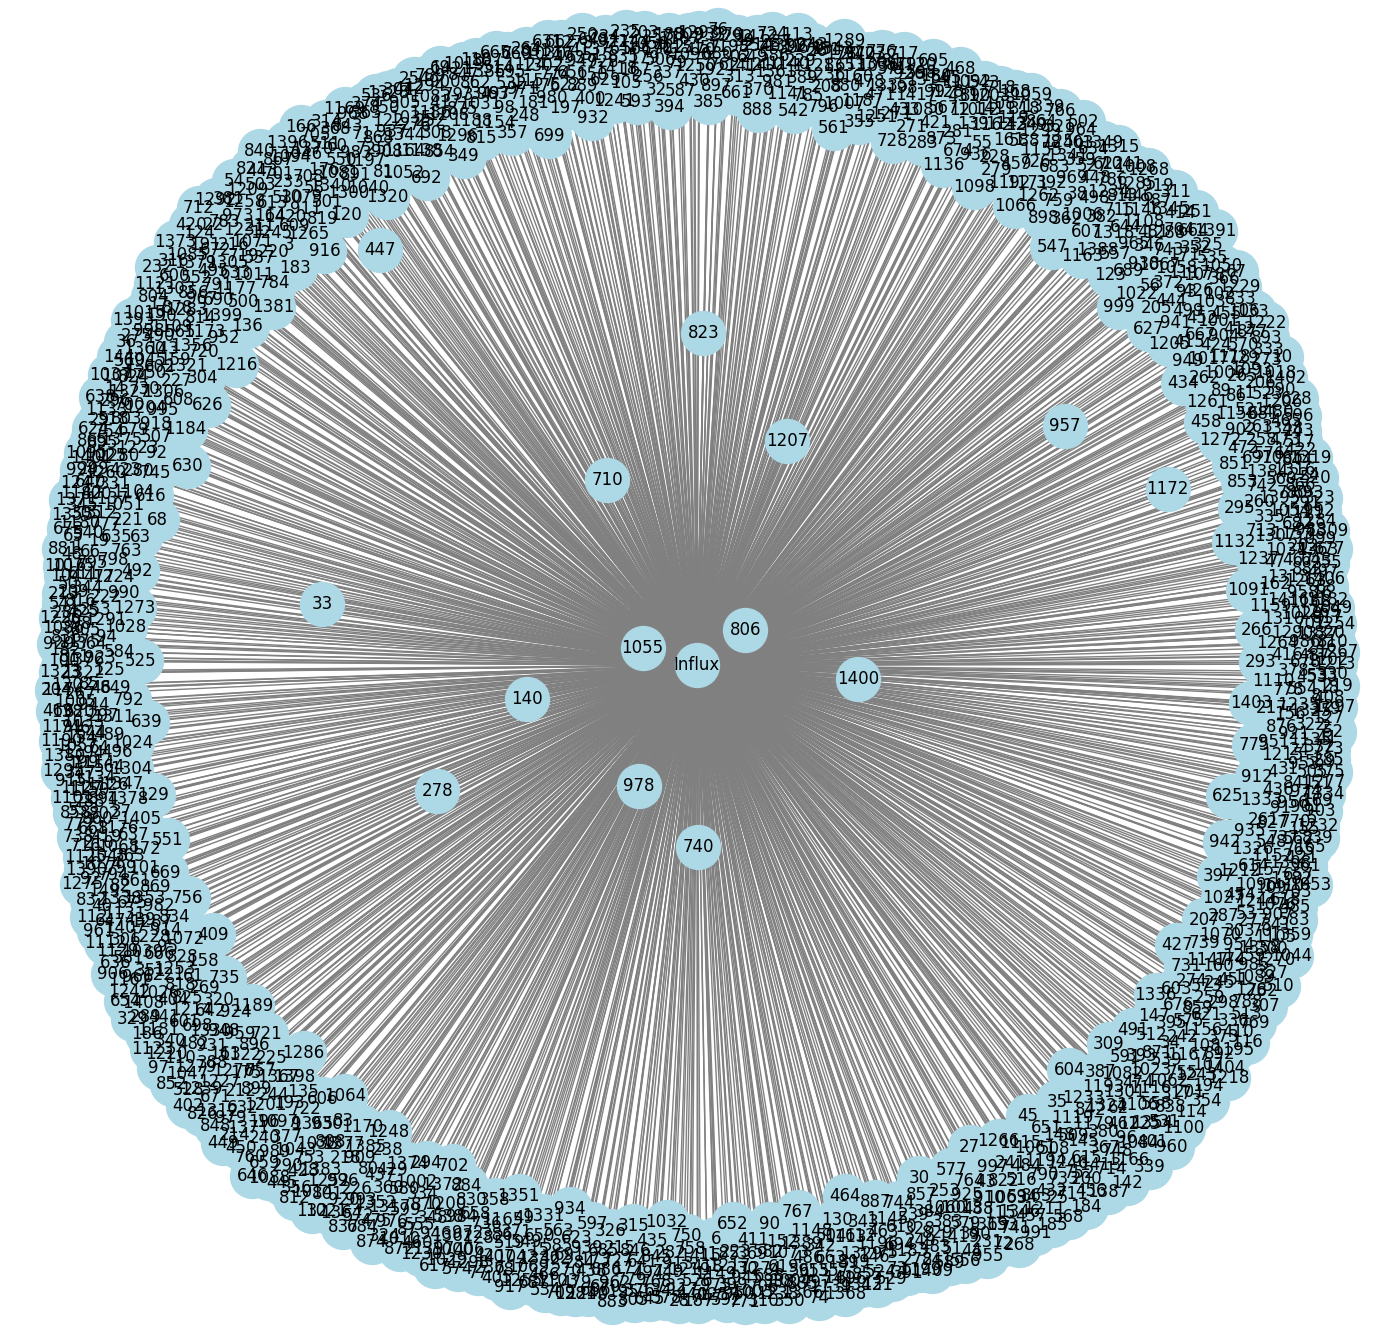
\includegraphics[height=.8\textheight]{assets/monitoring_system_architecture_2.png}
  \caption{Emmy's 1422 nodes located in G\"ottingen}
\end{figure}
\end{center}
\end{frame}

\section[Overview]{The Need for Speed: From Lucene to Grafana}
\begin{frame}{The Need for Speed: From Lucene to Grafana}
  \begin{itemize}
    \item We Evaluate Two Time-Series Databases:
    \begin{itemize}
      \item Elasticsearch, a distributed search engine.
      \item InfluxDB, a time-series database.
    \end{itemize}
  \item In order to understand why, one has to look at their shared history.
  \end{itemize}
\end{frame}

\begin{frame}
\begin{columns}[T]
\begin{column}{0.5\textwidth}
\begin{block}{Lucene}
\begin{itemize}
  \item Java-based Search Engine Library
  \item Developed in 1999 for Apache Nutch
  \item Fuzzy Full-Text Search
\end{itemize}
\end{block}
\begin{block}{Elasticsearch}
\begin{itemize}
  \item Distributed Search Engine
  \item Based on Lucene
  \item Developed in 2010
  \item Used at Wikipedia, Netflix, Stackoverflow, LinkedIn
\end{itemize}
\end{block}
\end{column}
\begin{column}{0.5\textwidth}
\vspace{1cm}
\begin{figure}
  
\includegraphics[width=\textwidth]{lucene.png}
  \caption{Lucene Logo}
  
\includegraphics[width=\textwidth]{elasticsearch.png}
  \caption{Elasticsearch Logo}
\end{figure}
\end{column}
\end{columns}
\end{frame}

\begin{frame}{Money, Money, Money}
\begin{itemize}
  \item Elasticsearch rose to popularity amongst the DevOps community.
  \item Thus, it grew beyond the scope of a hobby project and needed funding.
  \item And a database alone is not enough for business applications.
  \item Thus, the ELK stack was born.
\end{itemize}
\end{frame}

\begin{frame}{ELK(B) stack}
\begin{center}
\begin{figure}
  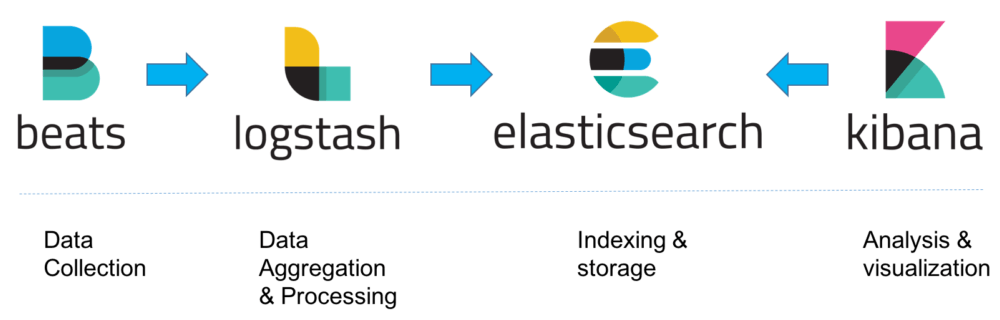
\includegraphics[width=\textwidth]{elk.png}
  % TODO: CITE https://www.michael-wutzke.de/elastic-stack-und-elasticsearch-grundlagen/
  \caption{ELK Stack}
\end{figure}
\end{center}
\end{frame}

\begin{frame}{Grafana}
\begin{columns}[T]
\begin{column}{0.5\textwidth}
\begin{itemize}
  \item System Monitoring Solution
  \item Forked from Kibana
  \item Specialized for time-series data
  \item Supports multiple data sources
  \begin{itemize}
    \item No Elasticsearch vendor lock-in
    \item Allows for more specialized database technologies
  \end{itemize}
\end{itemize}
\end{column}
\begin{column}{0.5\textwidth}
\begin{figure}
  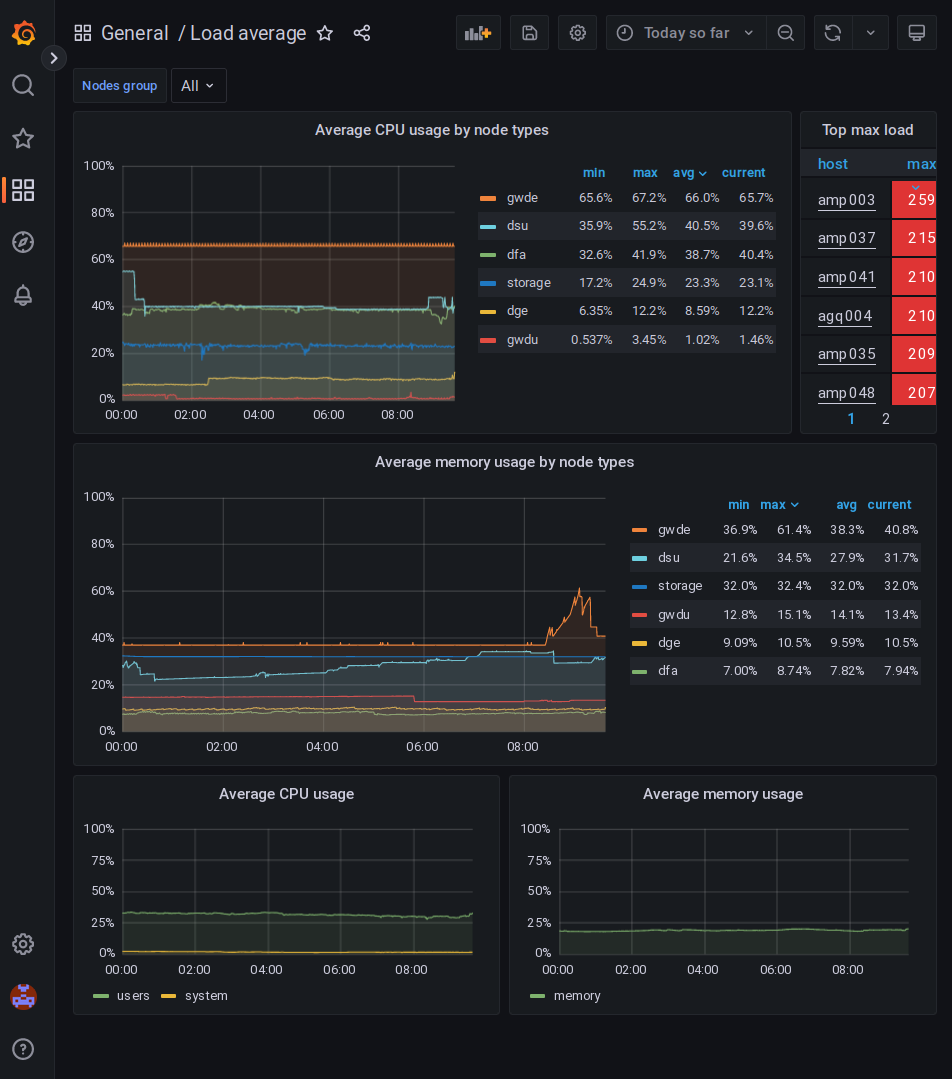
\includegraphics[height=.8\textheight]{example_grafana_dashboard.png}
\end{figure}
\end{column}
\end{columns}
\end{frame}

\begin{frame}{InfluxDB}
\begin{columns}[T]
\begin{column}{0.5\textwidth}
\begin{itemize}
  \item Time-Series Database
  \item Built for technology applications
  \item Highly specialized for time-series data
  \item Also used at the GWDG as a data source for Grafana
\end{itemize}
\end{column}
\begin{column}{0.5\textwidth}
\begin{figure}
  
\includegraphics[width=\textwidth]{influxdb.png}
  \caption{InfluxDB Logo}
\end{figure}
\end{column}
\end{columns}
\end{frame}

\section[Related Work]{Looking in the Rear-View-Mirror: Related Work}
\begin{frame}{Looking in the Rear-View-Mirror: Related Work}
\begin{columns}[T]
\begin{column}{0.5\textwidth}
\begin{itemize}
  \item Only a single exhaustive performance comparison of Elasticsearch and InfluxDB.
  \item Conducted by InfluxData, the company behind InfluxDB.
  \item Publically available on GitHub.
  \item In this section, we will deep dive into their methodology and findings.
  % TODO cite
\end{itemize}
\end{column}
\begin{column}{0.5\textwidth}
\begin{figure}
  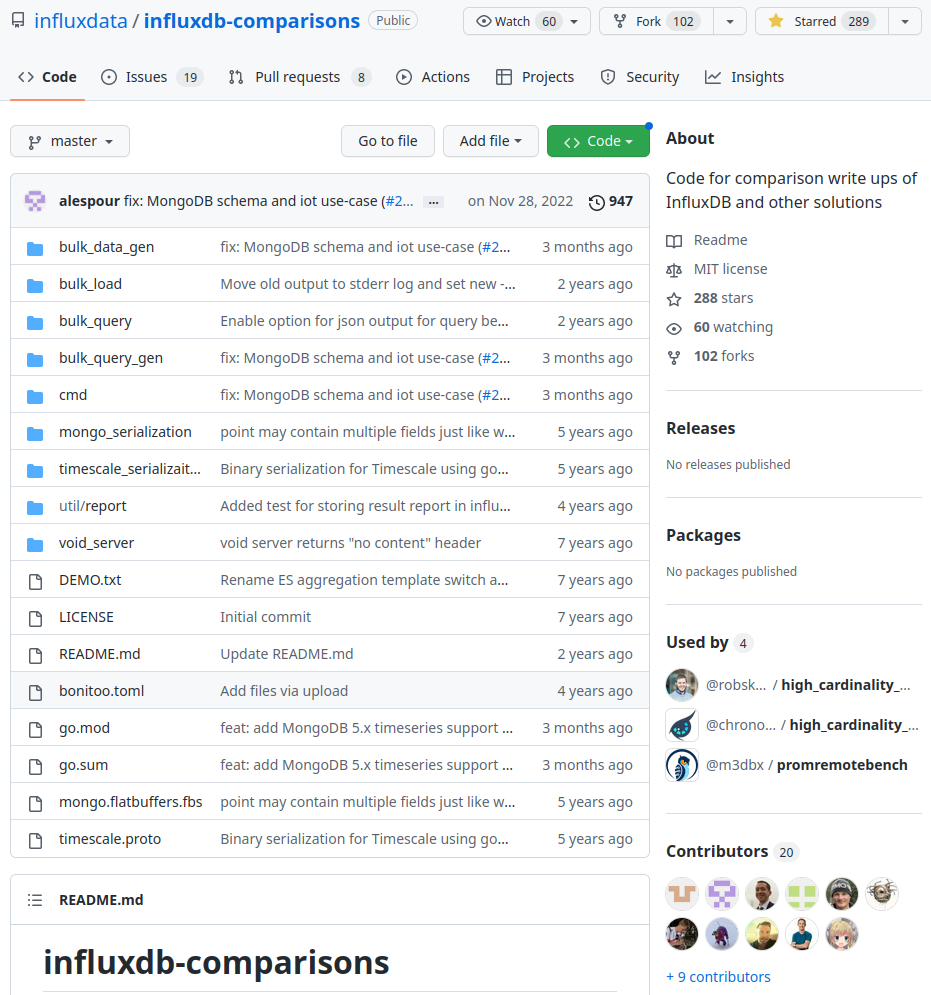
\includegraphics[height=.8\textheight]{github_influx.png}
\end{figure}
\end{column}
\end{columns}
\end{frame}

\begin{frame}{Overview}
\begin{itemize}
  \item Measured across 3 vectors
  \begin{enumerate}
    \item Data ingest performance
    \item On-disk storage requirements
    \item Mean query response time
  \end{enumerate}
\item Split into 5 disconnected steps
  \begin{enumerate}
    \item Data Generation
    \item Data Loading
    \item Query Generation
    \item Query Execution
    \item Query Validation
  \end{enumerate}
\end{itemize}
\end{frame}

\begin{frame}{Influx Comparisons}
\begin{block}{1. Data Generation}
\begin{itemize}
  \item Random and Deterministic (pinned PRNG seed)
  \item Shared generation logic
  \item Generated beforehand
  \item Modelled realistically
  \begin{itemize}
    \item DevOps related metrics, same structure as telegraf
    \begin{itemize}
      \item \texttt{cpu}, \texttt{diskio}, \texttt{kernel}, \texttt{mem}, \texttt{redis}...
    \end{itemize}
    \item clamped random walk
    \begin{itemize}
      \item important for optimizations such as delta compression
    \end{itemize}
  \end{itemize}
\end{itemize}
\end{block}
\end{frame}

\begin{frame}{Influx Comparisons}
\begin{block}{2. Data Loading}
  \begin{itemize}
    \item KISS
    \item Batched into bulk queries (default 5000 documents)
    \item parallelized (default 5 workers)
    \item sent as fast as possible
  \end{itemize}
\end{block}
\pause
\begin{block}{3. Query Generation}
  \begin{itemize}
  \item Random and Deterministic (pinned PRNG seed)
  \item Shared generation logic
  \item Generated beforehand
  \end{itemize}
\end{block}
\end{frame}


\begin{frame}{Influx Comparisons}
\begin{block}{4. Query Execution}
  \begin{itemize}
    \item KISS
    \item Sends parallelized range queries
  \end{itemize}
\end{block}
\pause
\begin{block}{5. Query Validation}
  \begin{itemize}
    \item Done via manual verification
    \item Ensuring that both aggregation results are approximately the same
  \end{itemize}
\end{block}
\end{frame}

\begin{frame}{Influx Comparisons}
\begin{block}{According to the White paper}
  % TODO QUOTE and cite
  \begin{itemize}
    \item InfluxDB outperformed Elasticsearch by \textbf{3.8x} when it came to data ingestion
    \item InfluxDB outperformed Elasticsearch by up to \textbf{7.7x} when measuring query performance
    \item InfluxDB outperformed Elasticsearch by delivering \textbf{9x} better compression
  \end{itemize}
\end{block}
\pause
\begin{block}{Problems}
\begin{itemize}
  \item Bad incentive structure
  \item Done with Influx version 1
  \item Not oriented for HPC workloads and topologies
  \item Data was ingested in bulk
\end{itemize}
\end{block}
\end{frame}

\section[Methodology]{Under the Hood: Our Methodology}
\begin{frame}{Under the Hood: Our Methodology}
  \begin{itemize}
    \item Extending InfluxData paper's methodology
    \item Everything not mentioned is the same.
    \item Adapted to our use case
    \begin{itemize}
      \item This is a huge feat; Emmy is big
      \item We run the recommended production configuration
      \item We mainly focus on write, not query read
      \begin{itemize}
        \item Since this is the bulk of the work
      \end{itemize}
    \end{itemize}
  \item Split into distinct phases as well.
    \begin{itemize}
      \item KISS! KISS! KISS!
    \end{itemize}
  \end{itemize}
\end{frame}

\begin{frame}{1. Data Generation}
\begin{itemize}
  \item Also random and deterministic, pinned PRNG seeds
  \item Only generating hardware / kernel measurements, no application metrics
  \item We use clamped 1D perlin noise
  \item One file per ingest worker!
  \begin{itemize}
    \item Less error prone!
    \item KISS!!!!!
  \end{itemize}
\end{itemize}
\end{frame}

\begin{frame}{2. Data Ingestion}
\begin{itemize}
  \item We don't use bulk ingestion
  \begin{itemize}
    \item instead, data of one node per request
  \end{itemize}
  \item Sending as fast as possible
  \item Flushing at the end
  \item Faster is better
\end{itemize}
\end{frame}

\begin{frame}{3. Check Index Compression}
  \begin{itemize}
    \item We do not trust their analytics
    \item Multi-Step process
    \begin{enumerate}
      \item Get size of data directory
      \item Fill the data
      \item Flush and Compress
      \begin{itemize}
        \item \textbf{InfluxDB}: Tree Compaction
        \item \textbf{Elasticsearch}: Force Merge API
      \end{itemize}
      \item After that, we measure again
    \end{enumerate}
    \item Smaller $\Delta$ is better
  \end{itemize}
\end{frame}

\begin{frame}{4. Design Queries}
\begin{columns}[T]
\begin{column}{0.5\textwidth}
\begin{block}{Methodology}
\begin{enumerate}
  \item Get a real world Grafana dashboard
  \item Extract the queries through the networking tab
  \item Port them to the Query Languages
  \item Make them parameterized
\end{enumerate}
\end{block}
\end{column}
\begin{column}{0.5\textwidth}
\begin{figure}
  \centering
  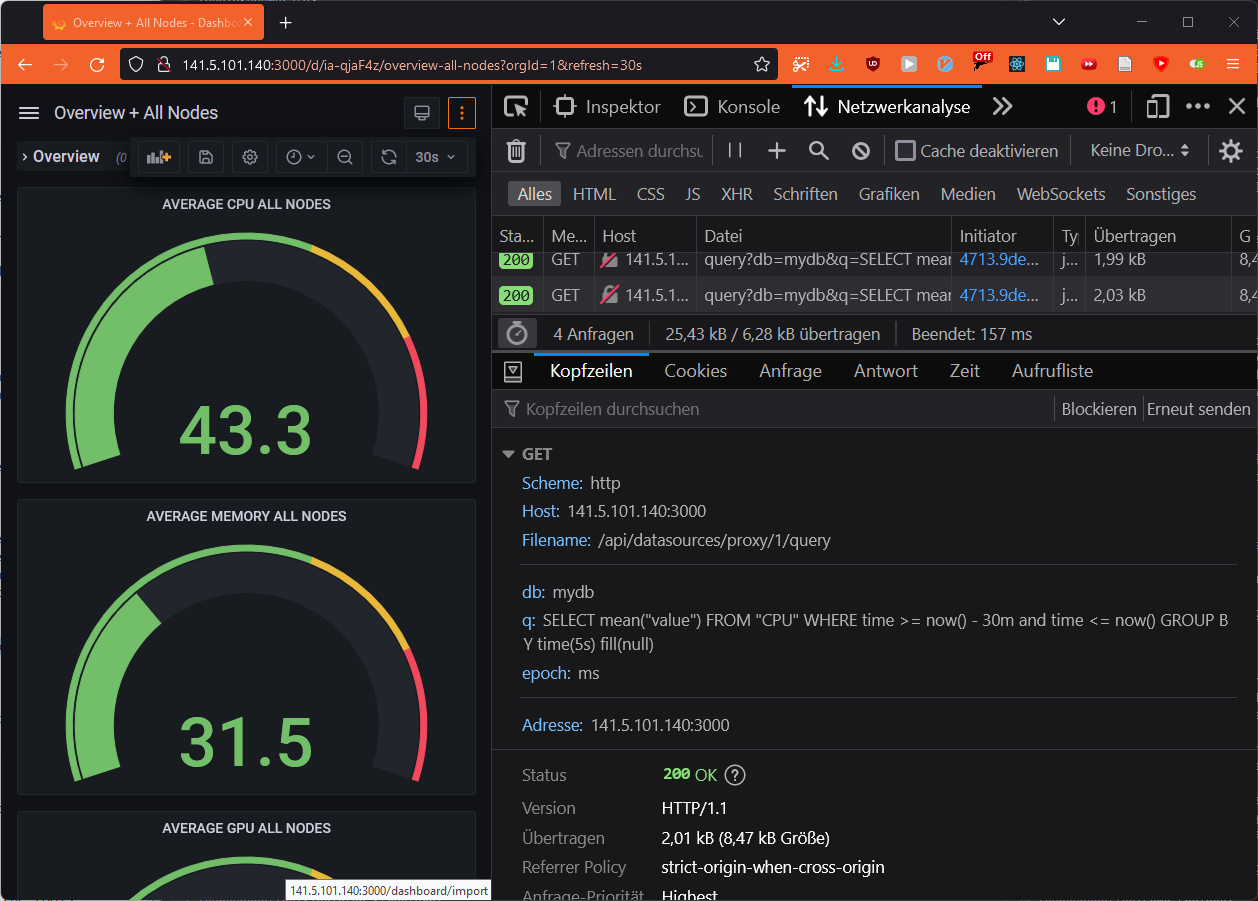
\includegraphics[width=\textwidth]{networking.png}
  \caption{Extracting through Networking Tab}
\end{figure}
\end{column}
\end{columns}
\end{frame}

\begin{frame}{5. Benchmark Queries}
\begin{itemize}
  \item We test querying while ingesting data
  \item Linear step increment of index size
  \begin{itemize}
    \item correllate the response time
  \end{itemize}
\item Faster is better
\end{itemize}
\end{frame}

\section[Results]{The Podium: Results and Conclusion}

\begin{frame}{The Podium: Results and Conclusion}
  \begin{center}
    \LARGE Stay tuned ;-)
  \end{center}
\label{pg:lastpage} % Label on last frame to get the page number for footer
\end{frame}

%\begin{frame}{References}
    % References slide in appendix
%    \renewcommand*{\bibfont}{\normalfont\scriptsize}
%    \printbibliography[heading=none]
%\end{frame}

\end{document}
